\chapter{User interface design}
\label{chap:user_interface_design}
Since our focus is on usability, the interface is the main body of our application. As our target audience is very wide, we have chosen to enforce an iterative development process, to be able to quickly response to new findings through e.g. usability tests.

\section{Wireframe}
\label{sec:wireframe}
By using the results from the analysis in chapter 2, we were at this point ready to start sketching an initial design. We started with the creation of a wireframe, which gave us an overview of how the different elements for the frontpage should be presented.

\begin{figure}[htb]
\begin{center}
\leavevmode
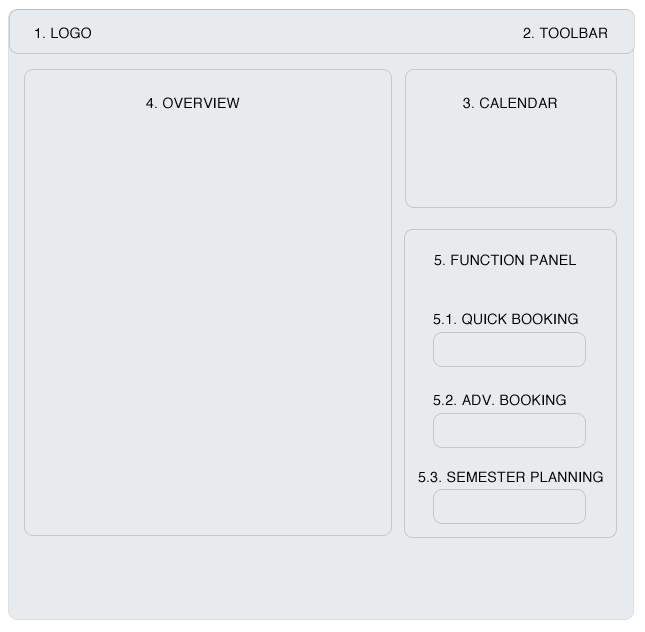
\includegraphics[width=0.6\textwidth]{images/wireframe1}
\end{center}
\caption{Wireframe for the frontpage}
\label{fig:wireframe_frontpage}
\end{figure}

\begin{itemize}
	\item \textbf{1. Logo}\\
	The logo for the application, which by convention should be located in the top left corner and link to the frontpage. \cite{steve}
	\item \textbf{2. Toolbar}\\
	A navigation toolbar. Should be used to login and logout, and for accessing the personal user account overview.
	\item \textbf{3. Calendar}\\
	An object used to navigate to a specific day in the future.
	\item \textbf{4. Overview}\\
	The main overview, which should present a map of the university.
	\item \textbf{5. Function panel}\\
	A panel containing buttons used to enter the booking interface, or the semester planning.
\end{itemize}

\section{Usability tests} % (fold)
\label{sec:usability_tests}
%%%% MENTION SOMETHING ABOUT SCENARIOS %%%%

% section usability_tests (end)


\section{Design process}
\label{sec:design_process}
To our project, the design of the graphical user interface is one of the most important things. Instead of focusing on hiding the difficulty of the problem by obscuring it with automisation and huge calculations, we seek to present suggestions and options for solutions in such a manner that a human being can lay the final touch. It has become apparent through our tests and interviews that no solution generated by a computer alone will be sufficient - there will always be conflicts needing a (to a computer) not obvious resolution, and even in the simplest of cases where no conflicts occur, human polish and/or acceptance is key.

We've undergone many iterations of each and every screen in the system, both those implemented in the prototype and those only on mockup stage. What follows is a tour through the process of the design.



\subsection{Narrowing the view}
The design of a page begins with deciding what tasks it should fulfil in our system, eg. a page to book a room for 2 hours. With that constantly in mind, we attempt to find all the possible things that particular function \emph{could} include. Some of them are extremely basic and obvious, eg. it needs to display which room you are booking, others are more complicated, as for example the ability to check whether a certain room is available on a regular basis, eg. every thursday between 9 and 11.

Through the process of brainstorming each page, we came up with smarter solutions to cover several different items on the could-list, or found out we needed a new page to handle all the advanced settings as an example. Once we had settled on the functionality of the page, we began piecing the puzzle together.



\subsection{Design of the day to day booking interface}
For a full history of our mockups, please refer to %\ref{app:mockups}

\begin{figure}[htb]
\begin{center}
\leavevmode
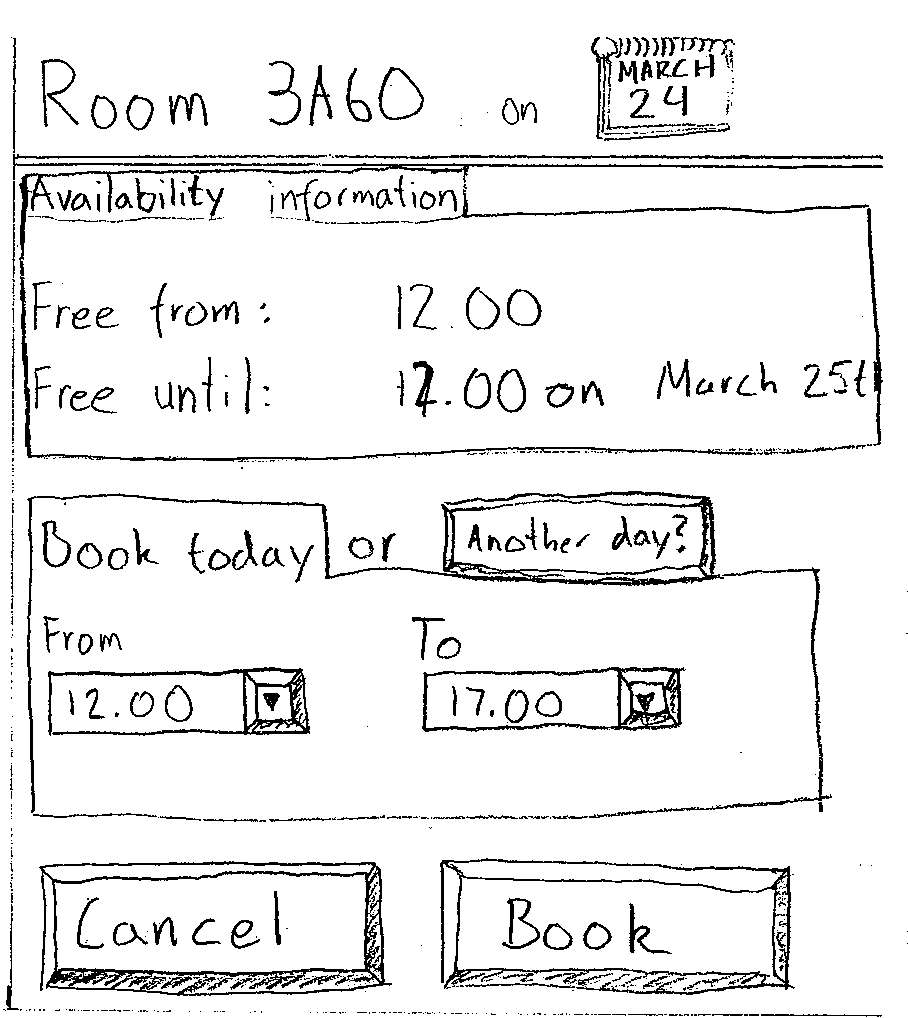
\includegraphics[width=0.6\textwidth]{images/bookRoomMockup}
\end{center}
\caption{First draft of the 'book room' panel}
\label{fig:book_room_mockup}
\end{figure}

Seen on figure \ref{fig:book_room_mockup} is the lower right panel of the main screen, which was thought to be in charge of all interaction, trying to give the user the impression that they never left the homepage, and to make sure no-one got lost in subscreens and menus. Our first usability tests quickly revealed that we had been mistaken. All the test subjects felt overwhelmed by the amount of options, and due to all the clutter did not spot the vital functions.

\begin{figure}[htb]
\begin{center}
\leavevmode
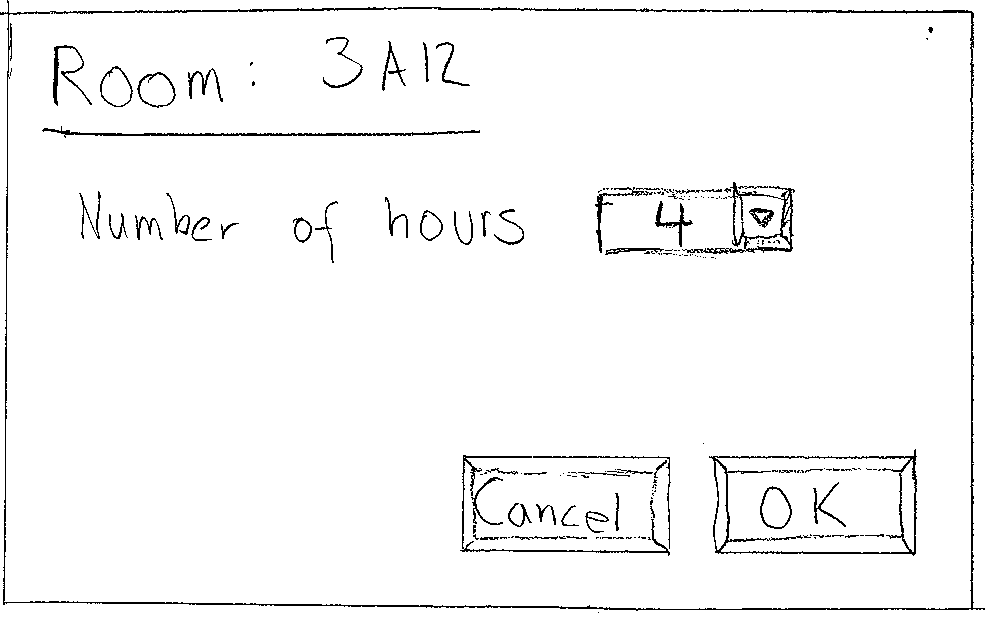
\includegraphics[width=0.8\textwidth]{images/bookRoomMockup2}
\end{center}
\caption{Second attempt at 'book room'. This time as a window overlaying the main view.}
\label{fig:book_room_mockup2}
\end{figure}

Second time around, we tried making it as basic as possible and simply presenting the user with a dialog (not a pop-up, just an overlay) for selecting how many hours from now the room should be booked. The flaw with this was that noone was able to figure out the availability of a room in the near future. This is when we realized that the best successes we've had with room booking was the first draft of the week-overview screen.

\begin{figure}[htb]
\begin{center}
\leavevmode
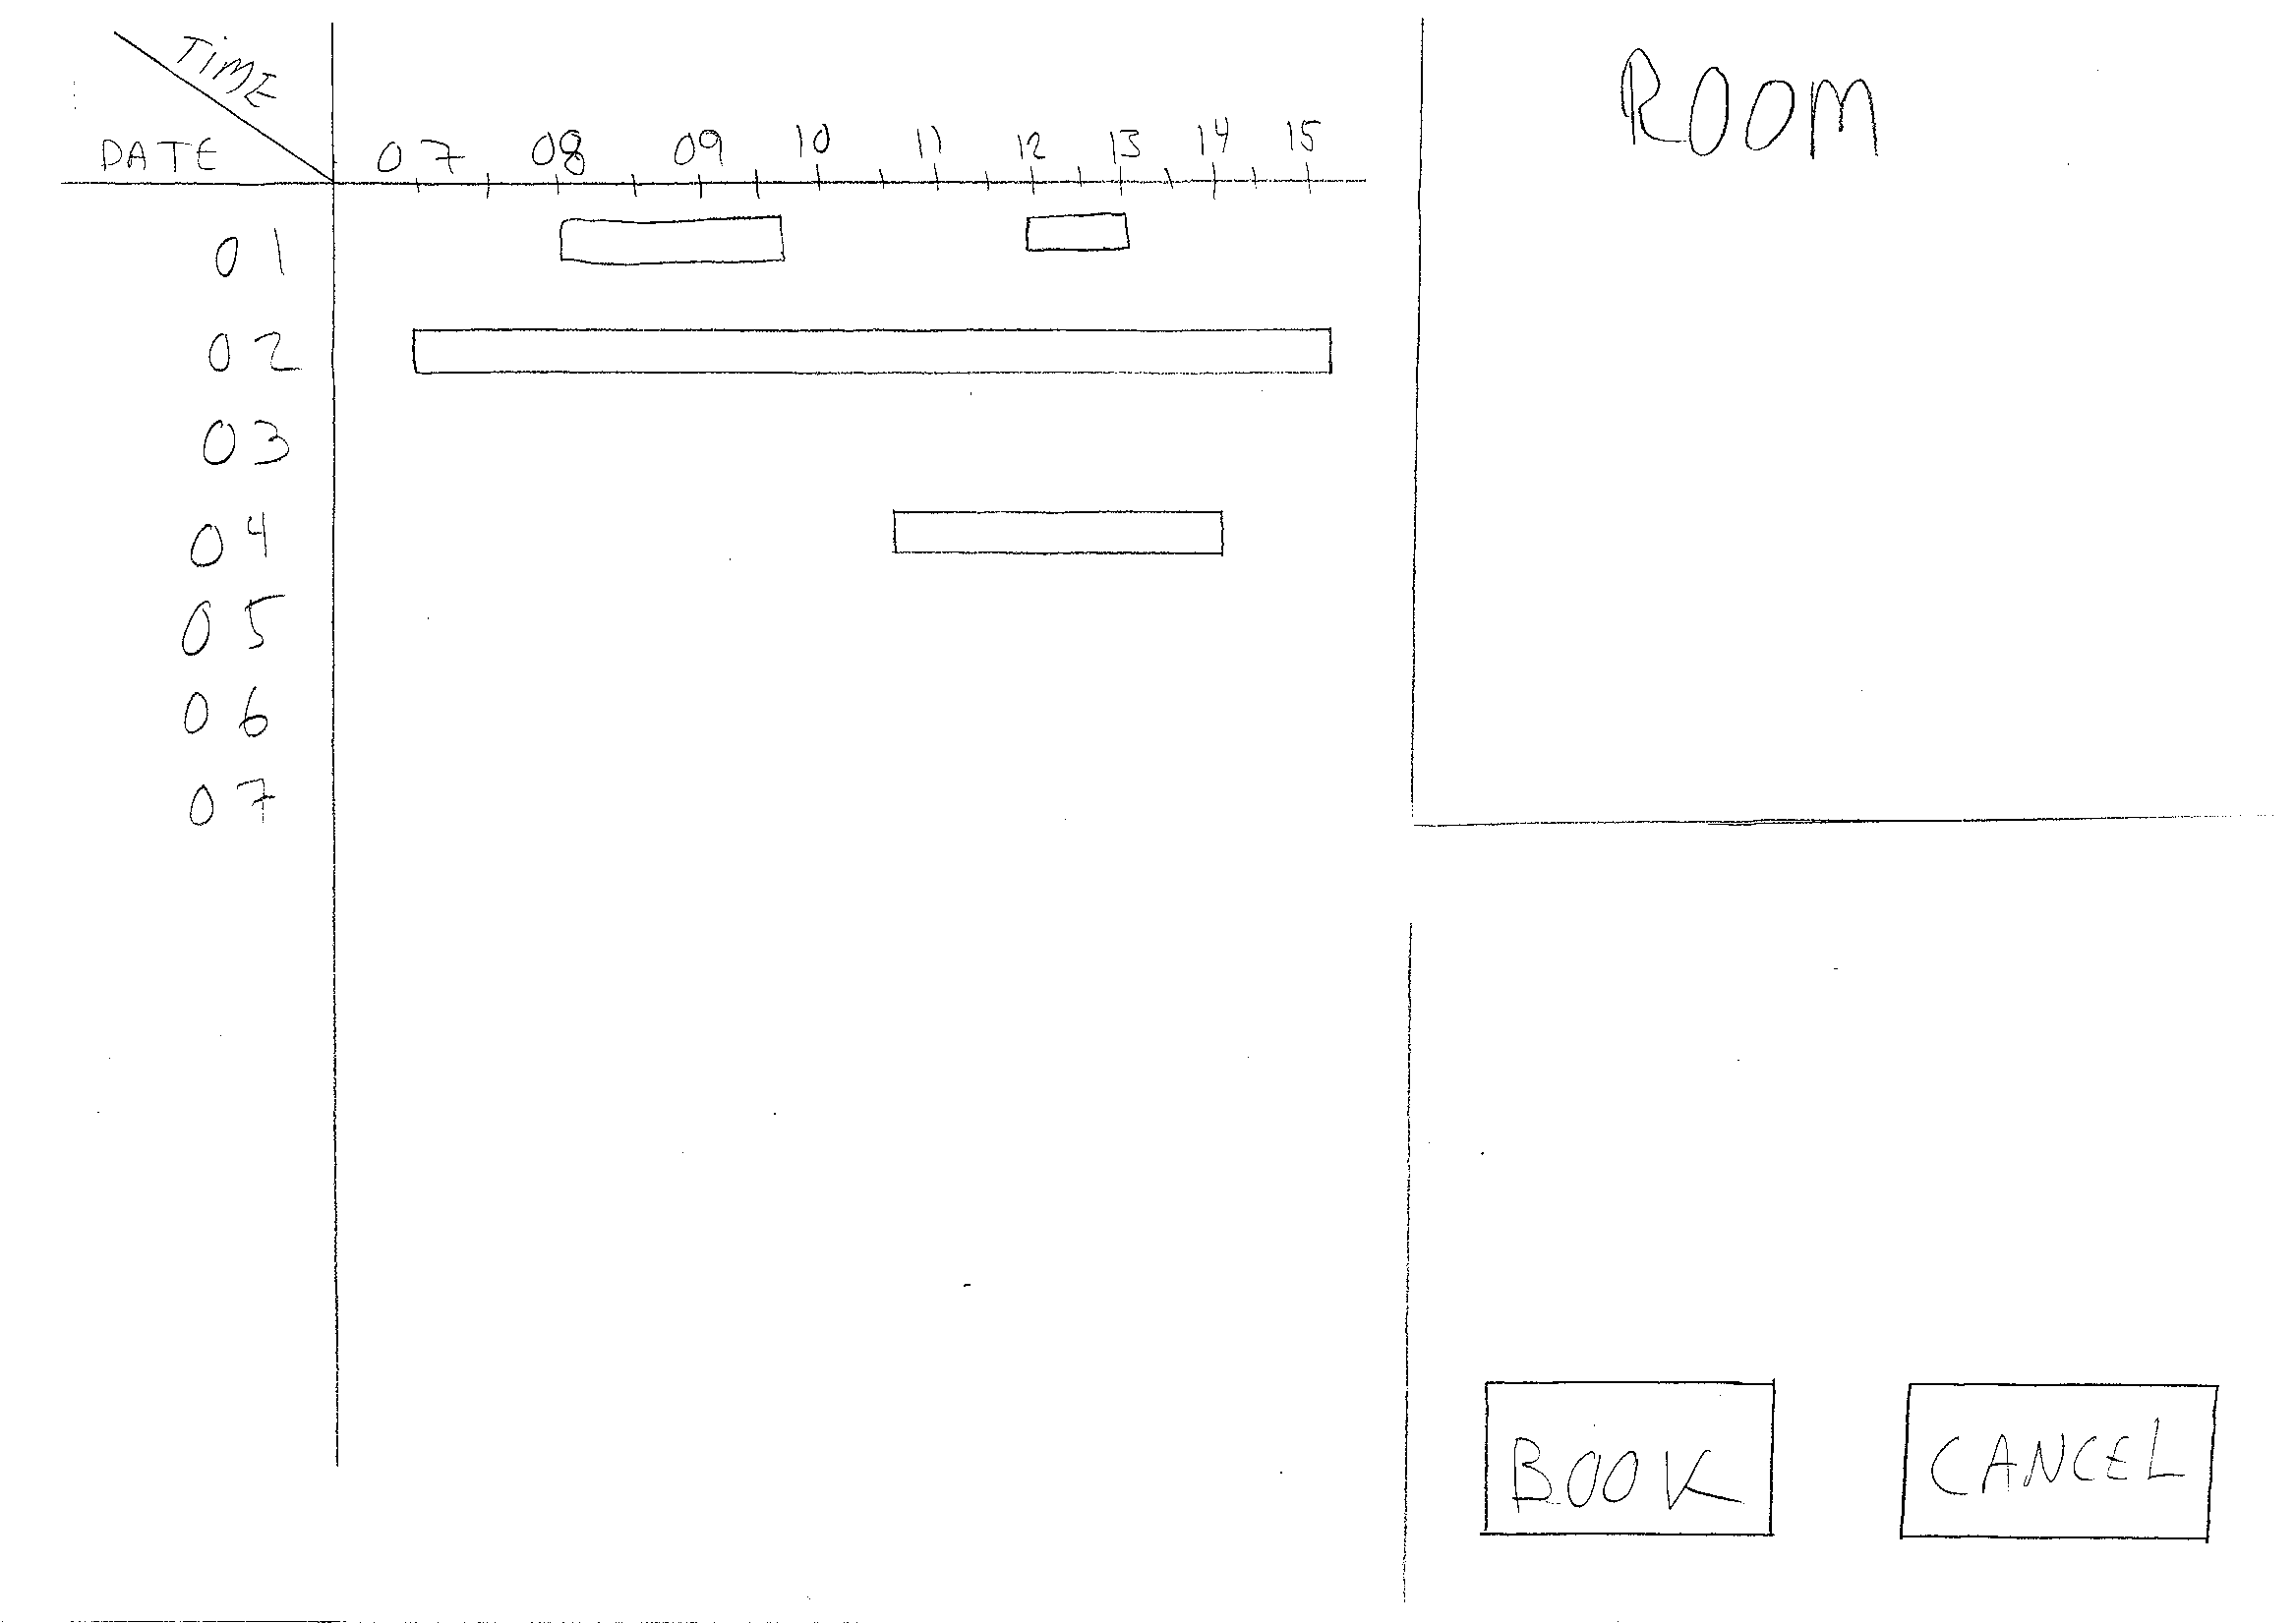
\includegraphics[width=0.8\textwidth]{images/weekMockup}
\end{center}
\caption{The mockup screen for a week overview on a specific room.}
\label{fig:week_mockup}
\end{figure}

All the test subjects used the 'matrix' overview shown on figure \ref{fig:week_mockup} both creatively and effectively, so we decided to try and utilize that success to the maximum by redirecting even a simple booking task to the same screen.
The only exception we have made to this is when using the "book now"-functionality, which will simply book a room for 4 hours and notify the user which one they have been assigned, with the ability to either accept or reject.

\begin{figure}[htb]
\begin{center}
\leavevmode
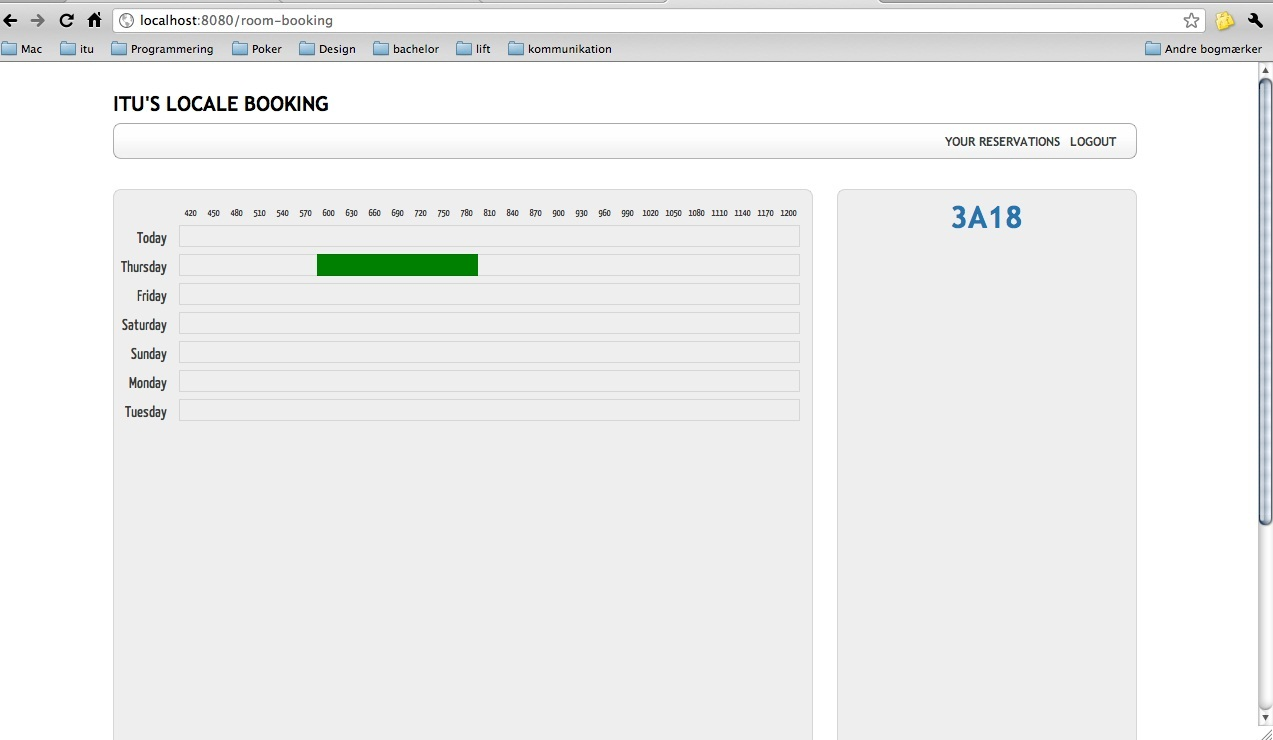
\includegraphics[width=1\textwidth]{images/weekFinal}
\end{center}
\caption{The almost finished screen for a week overview on a specific room.}
\label{fig:week_final}
\end{figure}

The final design to book a room, as shown on figure \ref{fig:week_final}, grants an availability overview of 7 days, starting with the current day. Through our tests, we noted test subjects trying to drag the mouse to select, and others clicking for a start time followed by a click on end time, so we have chosen to allow for both.
To assist the user in figuring out how it works, we have added highlighting of both the day and time when mouse is moved across the matrix.

Søren Lauesens first law of usability\cite{lauesen} states that a heuristic evaluation of usability flaws only has a 50\% hit-rate, which we admittedly found out was the case. We anticipated that our first design might be too dense, but never guessed that the wider overview proved more efficient for a simple booking.


\subsection{Layout}
%maybe move?
Being a website poses some extra considerations - namely those of browsing habits. Two examples we will refer to, and assume basic familiarity with, in this section are wikipedia.org and google.com
%kan dette bruges?
\todo{ indsæt små billeder af wikipedia og google med F-pattern eyetrack }

%Let us for a second imagine a search for 'random' was made on both those pages. According to research by Jakob Nielsen (---- indsæt ref), users tend to scan the page in a pattern slightly resembling a capital F, ignoring banners and everything that looks like 'off-site' content.

\section{Proposed design}
\label{sec:proposed_design}
\todo{Explain and illustrate the proposed design}
